
\chapter{Organisation du travail}


\section{Méthode de travail}

Nous avons cherché au mieux à répartir notre travail. Pour cela nous avons défini 3 grands axes de travail à l'issue de cette étude fonctionnelle.
\begin{itemize}
\item Dans un premier temps nous allons réaliser l'état de l'art.
\item Dans un deuxième temps nous étudierons la phase de réalisation.
\item Enfin nous testerons notre projet dans des conditions réelles.
\end{itemize}
~\\

Tout au long de ce projet nous avons choisi de réaliser notre travail en divisant notre équipe en 3 groupes de travail distincts formés respectivement de D'Acremont - Cotten, Legay - Rigaud, et Kenaan - Shehade. Notamment lors de l'état de l'art, ces groupes vont réaliser des recherches par binômes pour ensuite redistribuer les informations grâce aux outils mis à notre disposition (nous avons détaillé ces outils plus loin).
~\\

De plus, nous avons décidé lors de la phase de conception de diviser ce travail en plusieurs sous ensembles que nous définirons plus tard et qui seront chacun d'eux testés indépendamment, à l'image de tests unitaires en programmation.



\section{Outils utilisés}

Lors de notre projet nous avons choisi d'utiliser plusieurs outils de travail en collaboration.

\begin{itemize}
\item Nous utilisons \LaTeX~pour la rédaction de nos rapports.
\item Nous avons hébergé notre projet sur GitHub. Cela nous permet de travailler de manière collaborative avec un versionning.
\item Enfin nous utilisons un Framaboard du groupe Framasoft pour gérer les taches de notre projet.
\end{itemize}

~\\
~\\

\subsection{Framaboard}
\begin{center}
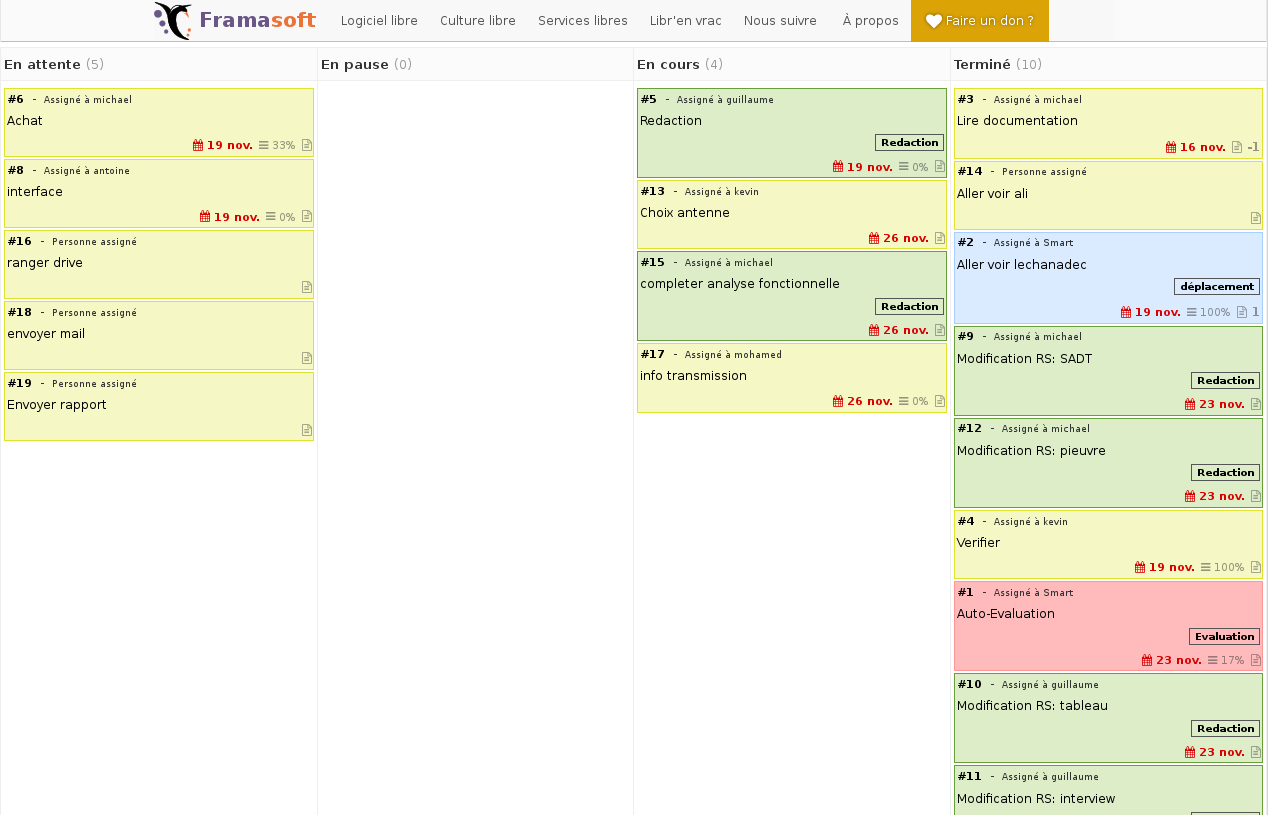
\includegraphics[width=0.9\textwidth]{framaboard}
\captionof{figure}{Impression d'écran de notre Framaboard}
\end{center}
Il est possible d'avoir accès en lecture à notre page Framaboard en cliquant  \textit{\href{https://smart.framaboard.org/?controller=board&action=readonly&token=ab1e20bb26472df067dc24cbd84d9b28eea71bfd68bdea07ab5a9b555ce0}{ici}}

\subsection{GitHub}
\begin{center}
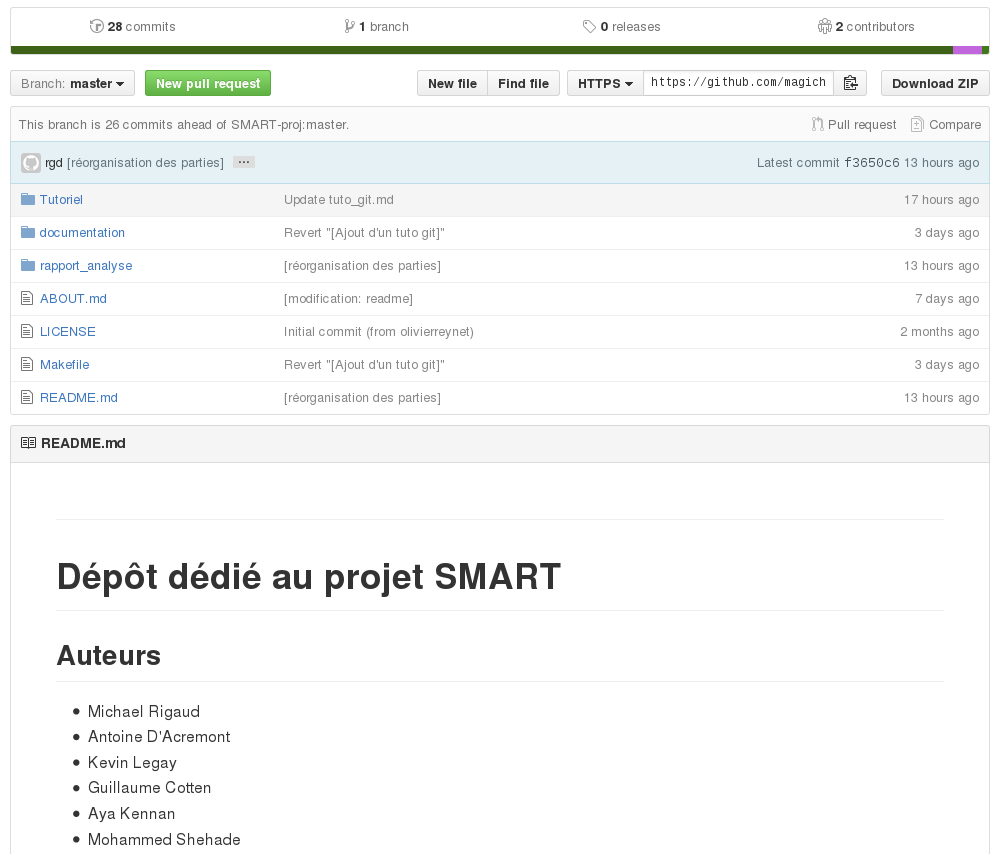
\includegraphics[width=0.9\textwidth]{github.png}
\captionof{figure}{Impression d'écran de notre GitHub}
\end{center}
Il est possible d'avoir accès à notre page GitHub en cliquant  \textit{\href{https://github.com/magichal/SMART}{ici}}


\newpage



\section{Diagramme de Grant}




%%% Local Variables: 
%%% mode: latex
%%% TeX-master: "../rapport"
%%% End: 
